% main.tex — CS348K final report
%
% Minimal wrapper so the section files compile standalone. If you already
% have a main.tex in Overleaf, just \input the section files from there or
% copy the body of section_1.tex into your existing document.
%
% Build:  pdflatex main && bibtex main && pdflatex main && pdflatex main

\documentclass[11pt]{article}

\usepackage[margin=1in]{geometry}
\usepackage{graphicx}
\graphicspath{{../assets/}{assets/}}
\usepackage{amsmath}
\usepackage{booktabs}
\usepackage{multirow}
\usepackage{caption}
\usepackage{subcaption}
\usepackage[round]{natbib}
\usepackage{hyperref}
\usepackage{xcolor}
\hypersetup{
    colorlinks=true,
    linkcolor=blue!50!black,
    citecolor=blue!50!black,
    urlcolor=blue!50!black,
}

\title{An Interactive Streaming Harness for Human Evaluation of\\Real-Time 3D Renderers}
\author{Connor Ding \texttt{<czsding@stanford.edu>} \\
        Ishita Gupta \texttt{<ishitagupta@stanford.edu>}}
\date{}

\begin{document}

\maketitle

% section_1.tex — Background and Setup

\section{Background and Setup}
\label{sec:background}

Novel View Synthesis (NVS) is an active area of research in 3D computer
graphics. The goal is to reconstruct a 3D representation of a scene from
a sparse collection of photographs taken from multiple camera angles.
Optimization-based approaches that fit either differentiable neural
fields~\citep{mildenhall2020nerf,mueller2022instantngp} or Gaussian
primitives~\citep{kerbl20233dgs} have advanced the field substantially
in both rendering quality and inference speed; we refer readers
to~\citet{tewari2022nrsurvey} for a comprehensive survey.

Defining ``good quality'' for a 3D rendering method is open-ended: the
final product is a visual artifact meant to be perceived by human eyes.
The literature predominantly relies on image-based metrics --- PSNR,
MS-SSIM, and LPIPS~\citep{zhang2018lpips} --- which compare reconstructed
views against ground-truth photographs held out from training. As
numerical distances these metrics are informative, but they have two
limitations in the 3D-rendering context:
\begin{enumerate}
    \item Two decades of image-quality work shows that good PSNR or
    MS-SSIM scores do not necessarily translate to a good perceptual
    experience~\citep{wang2009mse}. LPIPS partially addresses this with
    learned deep features but remains a proxy for direct viewing and is
    expensive to compute.
    \item Image-based metrics evaluate \emph{static} images at a small,
    fixed set of held-out camera poses, while users actually
    \emph{interact} with 3D scenes --- moving the camera, zooming, and
    viewing continuously from arbitrary angles. Free navigation
    introduces failure modes (popping, floater drift, smoothness
    artifacts at oblique angles) that no static-image metric can detect.
\end{enumerate}

To address this gap, we develop an interactive streaming harness for
human evaluation of real-time 3D renderers, built around the
philosophy that rendering quality should ultimately be measured by how
participants perceive it under interactive viewing. A researcher
supplies one or two renderers and a study configuration; the system
streams to participants' browsers, collects per-aspect ratings (and,
in two-method studies, an overall A/B preference with aspect
citations), and returns the raw per-participant data.

The system's inputs are a researcher-provided rendering algorithm and
its fitted 3D model, together with a study configuration (scenes,
conditions, protocol). Its outputs are the data collected from each
participant's session: (a)~\emph{subject ratings} produced through the
rating UI --- per-aspect 0--100 sliders, A/B preferences, and aspect
citations; (b)~\emph{free-text feedback} entered in the post-session
notes field; and (c)~\emph{mouse-movement trajectories} logged over
the participant's viewing window. The first two are the immediate
data products of the rating task; the third lets a researcher
reconstruct \emph{which views} of the scene each participant chose to
inspect before issuing a rating. Figure~\ref{fig:io} gives a
high-level view of how the system sits between the researcher and the
participant.

\begin{figure}[t]
  \centering
  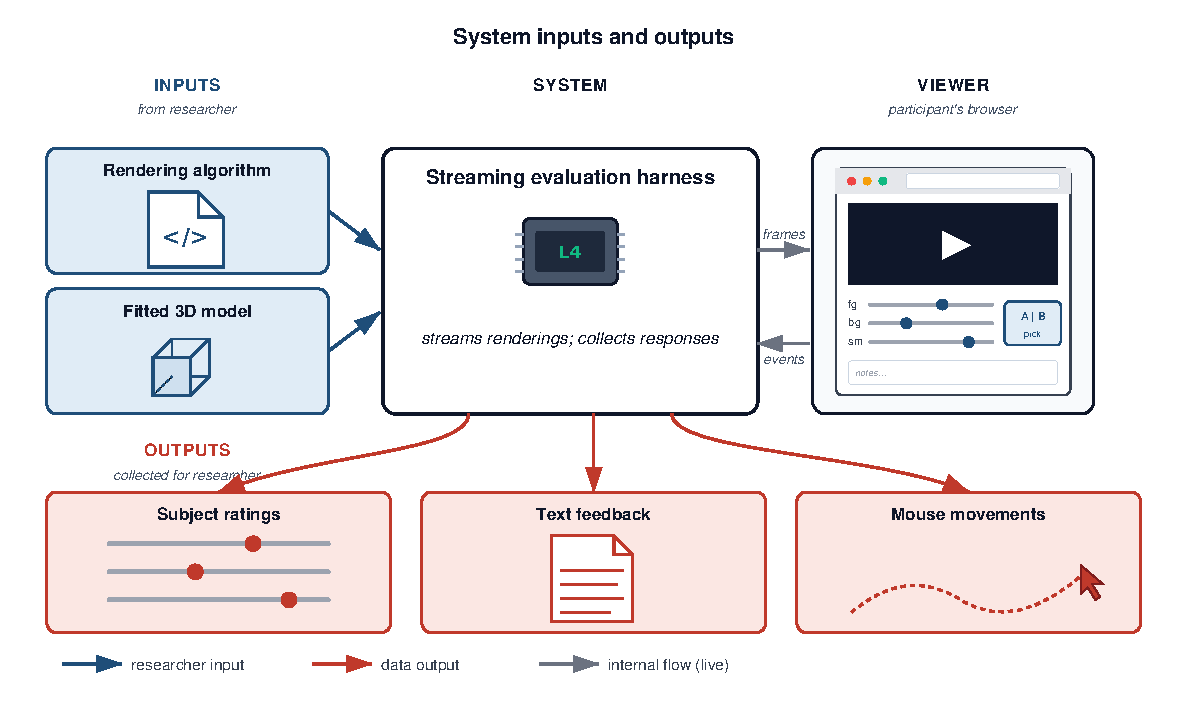
\includegraphics[width=\linewidth]{io_diagram}
  \caption{Conceptual view of system inputs and outputs. The researcher
  provides a rendering algorithm and a fitted 3D model; the system
  streams the resulting renderings to a participant's browser-based
  viewer and collects three categories of response data --- subject
  ratings, free-text feedback, and mouse-movement trajectories ---
  for the researcher to analyze.}
  \label{fig:io}
\end{figure}

The three \textit{main goals} are:
\begin{enumerate}
    \item Measure a dimension of rendering quality that image-based
    metrics on held-out static frames cannot capture: the participant's
    \emph{interactive perceptual experience} under continuous,
    free-roaming viewing. The collected data is intended as citable
    evidence a researcher can use to support claims about how their
    method actually behaves in interactive use, complementing rather
    than competing with the offline numbers already reported in the
    literature.
    \item Offer a plug-and-play framework where a researcher can connect
    their renderer and trained model and run a human study with minimal
    infrastructure work.
    \item Support both single-method subjective studies and two-method
    comparison studies, covering the two most common shapes of perceptual
    question a 3D-graphics researcher might ask.
\end{enumerate}
The three explicit \textit{non-goals} are:
\begin{enumerate}
    \item Replace image-based numerical metrics --- those metrics are
    cheap to compute, can be used as training losses, and remain the
    right tool for in-the-loop comparisons during method development.
    \item Modify the underlying rendering algorithms --- we provide a
    platform for evaluation, not for method improvement.
    \item Provide statistical analysis or visualization of the
    collected data --- the harness delivers raw per-participant
    response data; how that data is summarized, correlated against
    offline metrics, or visualized is the researcher's call.
\end{enumerate}
Two practical \textit{constraints} shape the system's design:
\begin{enumerate}
    \item \textit{Participants evaluate from their own machines},
    which we cannot assume to have GPUs capable of running an NVS
    renderer. The renderer must therefore run on a remote
    GPU-equipped instance, with the rendered output delivered to the
    participant's browser over the network. We host the active
    renderer(s) and supporting services on an AWS L4 GPU instance.
    \item \textit{The framework should be agnostic to the underlying
    rendering algorithm.} Different NVS methods use different
    rendering stacks --- CUDA-accelerated hash grids for i-NGP, a
    custom rasterizer for Nexels, the \texttt{gsplat} differentiable
    rasterizer for 3DGS --- and we want to support not just these
    three but whatever NVS method a future researcher brings. A
    framework that asked each renderer to ship its native output
    format to the browser would have to keep pace with every method's
    evolving toolchain. Streaming a common video format (H.264)
    abstracts that diversity away: every renderer emits the same
    output regardless of its internal representation.
\end{enumerate}
These constraints together motivate the streaming architecture
described in Section~\ref{sec:approach}.

To exercise the harness, we run two case studies of the kind a graphics
researcher might reach for when validating their own model. The first is
a single-viewpoint study --- participants view one rendering at a time
and rate it. The second is a two-viewpoint study --- participants compare
two NVS models side by side and select an overall preference along with
the aspects that drove that choice. The focus is on the system rather
than the findings of either case study; provided the resulting data are
coherent and non-degenerate, the harness has done its job.

A good evaluation harness must succeed on three independent axes.
\emph{System-side}: the streaming pipeline has to work end-to-end for a
diverse set of NVS methods. \emph{Researcher-side}: the data has to be
informative and analyzable on the researcher's own terms.
\emph{Participant-side}: each session has to feel smooth, clear, and
easy. We make all three criteria precise in
Section~\ref{sec:results}. The crux is twofold, and the methodological
half is the larger contribution. \emph{Methodologically}, we have to
design a questionnaire and a study protocol that meaningfully capture
interactive perceptual experience --- a design problem with no
off-the-shelf answer in the 3D-rendering literature, where every
existing instrument either reduces to an image-metric proxy or asks the
participant to rate a static frame. \emph{Infrastructurally}, we have
to deliver real-time renderings of multiple high-end NVS methods to a
remote browser at participant-imperceptible latency, on a single L4
GPU, with a renderer interface generic enough that adding a new method
does not require modifying the study logic.
Section~\ref{sec:approach} describes both;
Section~\ref{sec:results} reports the two case studies.

% section_2.tex — Approach (questionnaire design + streaming platform)

\section{Approach}
\label{sec:approach}

We start from existing third-party renderer implementations for the
three NVS methods we evaluate --- \texttt{pyngp} for
i-NGP~\citep{mueller2022instantngp},
\texttt{diff-nexel-rasterization} for Nexels~\citep{nexels}, and
\texttt{gsplat}~\citep{ye2024gsplat} for 3D Gaussian
Splatting~\citep{kerbl20233dgs}. What those projects do not ship is the
instrument: there is no agreed-upon questionnaire for asking a
participant how good a real-time 3D rendering feels, and no
off-the-shelf platform that runs such a questionnaire while the
participant interactively views a live render. The contribution of this
work is, in order of importance, the design of that questionnaire
(\S\ref{sec:questionnaire}) and the streaming harness that lets it run
(\S\ref{sec:platform}).

\subsection{Questionnaire design}
\label{sec:questionnaire}

\paragraph{Decomposing ``quality''.}
A single overall ``how good is this rendering'' rating is hard to
interpret across scenes and methods: it averages over different failure
modes, and the participant's internal weighting is opaque. We instead
decompose perceived quality into three sub-aspects that we elicit
separately:
\begin{enumerate}
    \item \emph{Foreground detail} --- sharpness and fidelity on the
    nominal subject of the captured photographs.
    \item \emph{Background detail} --- sharpness, fidelity, and absence
    of floater artifacts on the surrounding regions, which NVS methods
    tend to struggle with more than the foreground.
    \item \emph{Motion smoothness} --- continuity of the rendering during
    free navigation. This is the one aspect that \emph{requires}
    interactive viewing to evaluate at all.
\end{enumerate}
The first two are familiar from still-image quality work; the third is
the explicit reason this study exists as a streaming harness rather than
an image grader. The three axes also align with the kinds of design
tradeoffs an NVS researcher actually reasons about --- model capacity
allocated to subject vs.\ surroundings, and the speed cost of additional
parameters or splats.

\paragraph{Sliders rather than Likert.}
Each aspect is rated on a continuous 0--100 slider with the endpoints
labeled (``poor'' and ``excellent'') and the midpoint unlabeled. We
chose continuous sliders over a 5-point Likert scale for two reasons:
(i) sliders avoid the anchor-driven clustering that compresses Likert
distributions toward one or two modes, and (ii) on a 0--100 scale a
single within-participant slider can be correlated directly against an
offline metric on the same axis, which a 5-bucket categorical cannot.

\paragraph{Two-method comparison: independent viewports, forced A/B,
aspect citation.}
For the two-method comparison the participant sees two
\emph{independently orbitable} viewports side by side, with method
identities hidden behind anonymous badges (only the \texttt{test}
initials hook reveals them, and is never used in real sessions).
Independence is deliberate: a single baked camera trajectory would
dictate which artifacts the participant ever sees, but pilot sessions
confirmed that participants want to \emph{probe} the scene --- zooming
on suspicious regions, viewing the subject from oblique angles --- and
the artifacts they probe (popping, smoothness, floaters at grazing
angles) are precisely the ones a fixed trajectory would either hide or
showcase. After exploring a pair, the participant fills out per-side
foreground / background / smoothness sliders, then makes a forced A/B
overall preference (``A'', ``B'', or explicit tie), then selects from a
multi-select list \emph{which} aspect(s) shaped that choice. The
slider-then-A/B redundancy is intentional: we collect both a graded
within-method rating and a categorical between-method judgment per
trial, and the aspect multi-select converts an aggregate preference
into something mechanistic --- which aspect, on which scene, swung the
choice.

\paragraph{Single-method convergence: ratings in isolation, reference
anchor.}
The convergence case uses the same primitives in a different shape. The
participant sees one viewport, rendering one stimulus (here: a 3DGS
checkpoint at a given training-iteration count) at a time; the active
stimulus is swapped without a process restart, so the only thing that
changes between consecutive stimuli is the model state. We deliberately
rate each stimulus in isolation rather than as A/B against the previous
one, since the stimuli are not always commensurable on a single axis of
merit and a forced choice would discard graded information. Per
stimulus we collect two sliders --- overall quality and motion
smoothness --- on the same 0--100 scale as the comparison case. To
give the participant a ground-truth anchor for what the scene
\emph{should} look like, we play a low-frame-rate slideshow of the
training photographs for the scene once before its rating block; an
NVS rendering on its own provides no reference for ``how detailed
should this actually be''.

\subsection{Streaming platform}
\label{sec:platform}

The streaming pipeline exists to let either questionnaire above run
while the participant views a live render rather than a pre-baked
trajectory, despite participants connecting from their own
(typically GPU-less) laptops, and despite the underlying renderers
having different native rendering stacks --- the two constraints
flagged in \S\ref{sec:background}. The platform is, by intent, the
smaller half of the contribution: it is what allowed us to ship the
questionnaire, not a research artifact in itself.

\paragraph{Pipeline.}
Each renderer is wrapped in a thin process
(\texttt{interactive\_renderer.py},
\texttt{nexels\_renderer.py}, \texttt{gsplat\_renderer.py}) that
consumes camera-pose deltas on a per-method WebSocket and pushes H.264
over RTSP to a \texttt{mediamtx} instance, which relays to the browser
over WebRTC (WHEP). A single browser-facing WebSocket multiplexer
(\texttt{ws\_mux.py}) routes pose-delta messages to the right renderer
based on URL path, and a static HTTP server (\texttt{serve.py}) hosts
the viewer pages and accepts rating submissions. All server-side
processes colocate on a single AWS L4 GPU instance.
Figure~\ref{fig:architecture} shows the resulting data flow.

\begin{figure}[t]
  \centering
  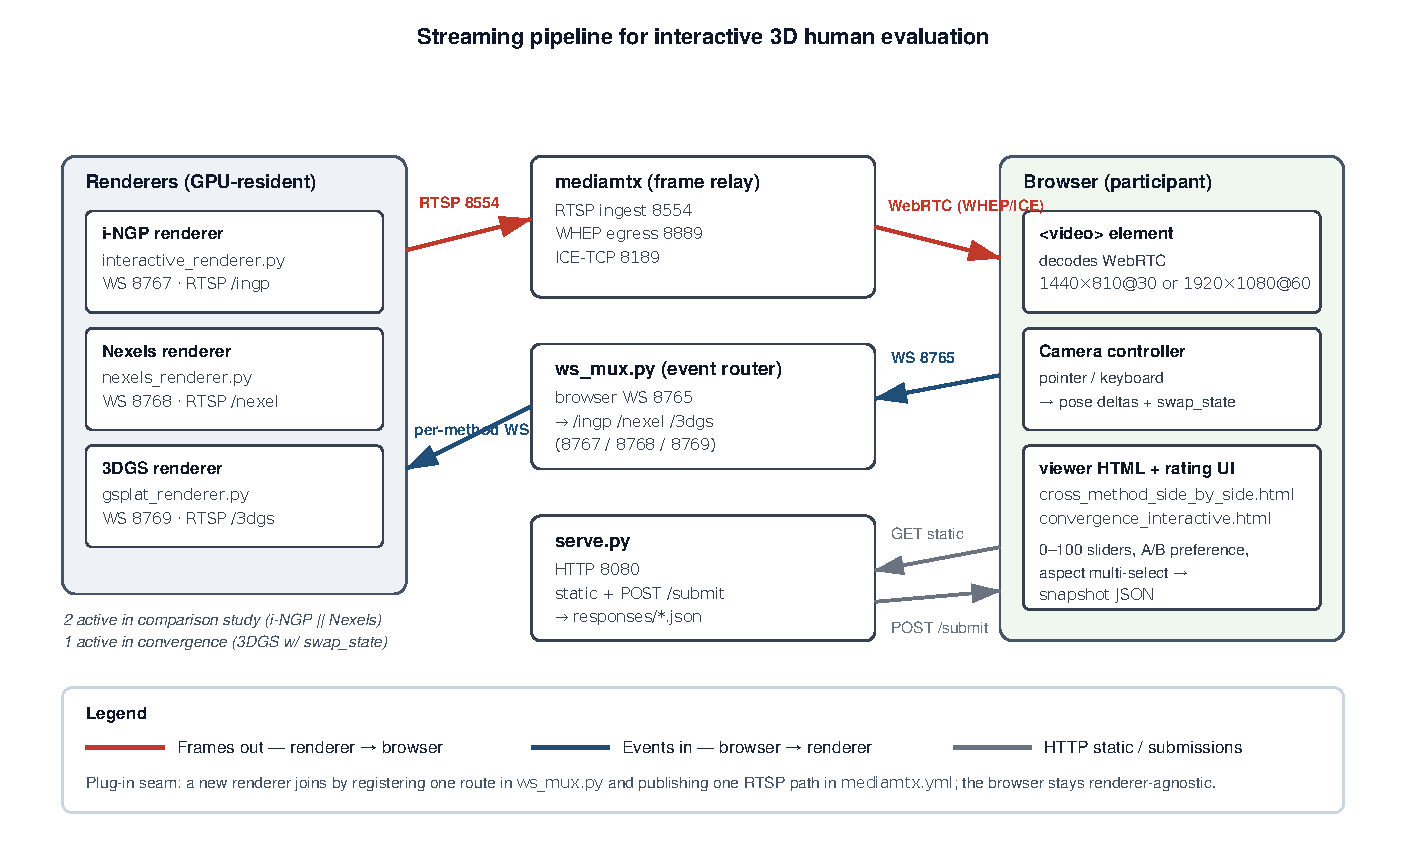
\includegraphics[width=\linewidth]{architecture}
  \caption{Streaming pipeline. The three renderers conform to a common
  contract (RTSP push for frames out, per-method WebSocket for events
  in); \texttt{ws\_mux.py} and \texttt{mediamtx} between them keep the
  browser renderer-agnostic.}
  \label{fig:architecture}
\end{figure}

\paragraph{Plug-and-play seam.}
The principal design choice on the platform side is the contract every
renderer must satisfy: (a) accept camera-pose deltas as JSON messages
on a per-method WebSocket port; (b) push H.264 over RTSP at the
configured target resolution and frame rate (1440$\times$810@30 for the
comparison case, 1920$\times$1080@60 for the convergence case); and
(c) optionally accept a \texttt{swap\_state} message used by the
convergence case to flip the active checkpoint without restarting the
renderer process. Any process that meets this contract drops in by
registering a route in \texttt{ws\_mux.py} and a corresponding RTSP
path in \texttt{mediamtx.yml}. The browser never has to know which
underlying method is active --- the same viewer HTML works for any
renderer that honors the contract, and the marginal cost of adding a
third method is a few lines of configuration rather than a viewer
rewrite.

\paragraph{What did not work.}
Two earlier designs are preserved in \texttt{archive/}. A fully
pre-rendered evaluation built on canned camera trajectories rendered to
MP4 surfaced the exact limitation that motivated the streaming
approach --- participants could not probe the artifacts they wanted to
talk about. A second attempt used Xvfb plus each renderer's native UI,
with \texttt{event\_relay.py} translating browser events into
\texttt{xdotool} keystrokes; this worked end-to-end but the
screen-capture path added tens of milliseconds, and the design did not
generalize to running two renderers concurrently because each demanded
its own X display. The current architecture replaced both.

% section_3.tex — Evaluation and Results
% Current participant counts: cross-method n=18, convergence n=12.

\section{Evaluation and Results}
\label{sec:results}

\subsection{Definition of success}
\label{sec:success}

A useful evaluation harness has to satisfy two parties, as flagged at
the end of \S\ref{sec:background}. We restate the two criteria here in
concrete, checkable form.

\paragraph{Researcher-side success.}
The harness should give a graphics researcher data they can act on
without engineering the data pipeline themselves. Concretely:
(a)~every participant who starts a session leaves a snapshot JSON on
disk, including sessions that ended early; (b)~the resulting data has
informative structure --- within-participant slider spread is
non-trivial, A/B preferences are not all ties, and aspect citations
are distributed across the three options rather than degenerate on one;
and (c)~the data shape is general enough that a researcher can apply
analyses of their own choosing (correlations against offline metrics,
within-trial regressions, inter-rater agreement) without bespoke
parsing.

\paragraph{Participant-side success.}
The session should feel smooth and easy to complete. Concretely:
(a)~interactive latency is below the threshold at which participants
notice it as ``laggy''; (b)~both renderers sustain their target frame
rate over the full session without sustained dips; (c)~no participant
abandons mid-session for technical reasons; and (d)~the rating UI is
clear enough that no experimenter intervention is required.

Participant-side success is harder to measure than researcher-side
success because it is partly experiential: systems telemetry can
confirm that no frames were dropped, but it cannot confirm that the
participant felt the session was pleasant. We rely on telemetry as an
indirect proxy for now, and plan to administer a brief post-session
self-report survey (in preparation) covering perceived smoothness,
clarity of the rating UI, and fatigue (\S\ref{sec:participant_feedback}).
The dual-party framing also clarifies what kind of failure invalidates
what kind of conclusion: a participant-side failure (frame stalls, UI
confusion) propagates into researcher-side measurements and invalidates
them, while a researcher-side data-shape ``failure'' --- sliders all
pegged at one end, for instance --- could itself be a valid measurement
of a real ceiling effect rather than a harness bug.

\subsection{Case studies}
\label{sec:setup}

We exercised the harness with two case studies. Both ran on a single
AWS GPU instance with an NVIDIA L4 (24~GB VRAM, \texttt{g6.xlarge}),
hosting all server-side processes (\texttt{mediamtx}, \texttt{ws\_mux},
\texttt{serve.py}, and the active renderers) on the same host.
Participants connected from their own machines over the public
internet; we did not constrain network conditions or display
characteristics, and we discuss the resulting variance in
\S\ref{sec:limitations}. Across both studies we recruited 19 unique
participants from the authors' friends and labmates; eleven of the
twelve case-B participants had previously completed case A. A case-A session
lasted a median of 9~minutes (mean 10); a case-B session a median of
5~minutes. We collected $n=18$ complete sessions in case study A and
$n=12$ in case study B; recruitment is closed for this submission.

\paragraph{Case study A: comparison (i-NGP vs Nexels).}
Two NVS methods --- i-NGP and Nexels --- rendered side-by-side at a
matched storage budget ($\approx$14~MB per scene; see
Table~\ref{tab:cross_offline}) over six mip-NeRF-360 scenes
(\texttt{bicycle}, \texttt{counter}, \texttt{garden}, \texttt{kitchen},
\texttt{room}, \texttt{stump}) plus one practice scene
(\texttt{bonsai}). The two methods stream concurrently to two
side-by-side viewports at 1440$\times$810@30. Method identity is
hidden on the viewport badges (only the \texttt{test} initials hook
reveals it, and is never used in real sessions). The seven scene pairs
are presented in a per-participant random order; side assignment of
i-NGP and Nexels is coin-flipped per pair; the first pair
(\texttt{bonsai}) is the practice trial and is excluded from analysis.
The questionnaire shape --- per-side sliders, forced A/B, aspect
multi-select --- is described in \S\ref{sec:questionnaire}.

\paragraph{Case study B: convergence (3DGS at four checkpoint counts).}
A single method (3D Gaussian Splatting) trained for varying numbers of
iterations (1k, 3k, 7k, 30k) on two Tanks-and-Temples scenes
(\texttt{train}, \texttt{truck}) --- eight stimuli total. All eight
checkpoints are GPU-resident ($\approx$1.4~GB combined, 210k--3.8M
splats per checkpoint), so swapping the active checkpoint is a
constant-time pointer update. The renderer streams 1920$\times$1080@60.
Before each scene's rating block, the participant watches a
low-frame-rate slideshow of the training photographs as a
ground-truth reference. Scene order is randomized; iteration order
within a scene is fixed ascending so the reference frame for
\emph{better} stays stable across the four levels.

\paragraph{Offline-metric baselines.}
For each scene--method pair in case study A and each
scene--checkpoint pair in case study B we computed PSNR, SSIM, and
LPIPS on the held-out test split for that scene (mip-NeRF-360
hold-every-eighth-view convention for case study A; gsplat
validation split for case study B). LPIPS uses the AlexNet backbone in
both cases for consistency. Tables~\ref{tab:cross_offline}
and~\ref{tab:convergence} list these per-stimulus offline numbers
alongside the corresponding mean slider scores.

\begin{table}[t]
\begin{minipage}[t]{0.48\textwidth}
\centering\footnotesize
\captionof{table}{Case study A: \emph{offline metrics} at the
\texttt{small} size setting ($\approx$14~MB per scene). PSNR / SSIM /
LPIPS are computed on the held-out mip-NeRF-360 test split with a
consistent LPIPS-AlexNet backbone; FPS is from each method's bench
script over 200 cycled test-camera frames at 1297$\times$840. Bold
marks the per-scene winner on each column. \texttt{bonsai} is the
practice scene and is excluded from the mean.}
\label{tab:cross_offline}
\setlength{\tabcolsep}{3pt}
\begin{tabular}{llrrrrr}
\toprule
Scene & Method & PSNR$\uparrow$ & SSIM$\uparrow$ & LPIPS$\downarrow$ & FPS & MB \\
\midrule
bicycle & i-NGP  & 21.93          & 0.462          & 0.592          & \textbf{62.0} & 14.5          \\
        & Nexels & \textbf{22.21} & \textbf{0.539} & \textbf{0.424} & 29.5          & \textbf{14.4} \\
counter & i-NGP  & 25.31          & 0.757          & 0.272          & \textbf{61.5} & \textbf{13.5} \\
        & Nexels & \textbf{26.42} & \textbf{0.833} & \textbf{0.216} & 30.0          & 14.4          \\
garden  & i-NGP  & 23.13          & 0.514          & 0.456          & \textbf{74.9} & \textbf{12.0} \\
        & Nexels & \textbf{23.46} & \textbf{0.636} & \textbf{0.322} & 34.0          & 14.4          \\
kitchen & i-NGP  & 27.12          & 0.767          & 0.214          & \textbf{96.2} & \textbf{12.6} \\
        & Nexels & \textbf{27.68} & \textbf{0.861} & \textbf{0.167} & 31.9          & 14.4          \\
room    & i-NGP  & 28.47          & 0.844          & 0.225          & \textbf{69.8} & 15.0          \\
        & Nexels & \textbf{29.15} & \textbf{0.877} & \textbf{0.207} & 29.8          & \textbf{14.4} \\
stump   & i-NGP  & 21.68          & 0.473          & 0.574          & 27.0          & 16.0          \\
        & Nexels & \textbf{23.88} & \textbf{0.604} & \textbf{0.398} & \textbf{32.9} & \textbf{14.4} \\
\midrule
\multirow{2}{*}{\textbf{mean}}
        & i-NGP  & 24.61          & 0.636          & 0.389          & \textbf{65.2} & 13.9          \\
        & Nexels & \textbf{25.47} & \textbf{0.725} & \textbf{0.289} & 31.4          & 14.4          \\
\bottomrule
\end{tabular}
\end{minipage}
\hfill
\begin{minipage}[t]{0.48\textwidth}
\centering\footnotesize
\captionof{table}{Case study A: \emph{per-scene human ratings}
($n=18$ participants). \textbf{fg}, \textbf{bg}, \textbf{sm} are mean
0--100 slider scores for foreground, background, and rendering
smoothness. \textbf{Votes} is the number of participants who preferred
that method on that scene; tie counts are bicycle 3, counter 1,
garden 4, kitchen 2, room 1, stump 1. Bold marks the per-scene winner
on each column.}
\label{tab:cross_human}
\setlength{\tabcolsep}{4pt}
\begin{tabular}{llrrrr}
\toprule
Scene & Method & fg$\uparrow$ & bg$\uparrow$ & sm$\uparrow$ & Votes \\
\midrule
bicycle & i-NGP  & 73.3          & 46.4          & 66.6          & 2              \\
        & Nexels & \textbf{80.6} & \textbf{68.3} & \textbf{72.5} & \textbf{13}    \\
counter & i-NGP  & \textbf{68.6} & 54.9          & \textbf{55.4} & 6              \\
        & Nexels & 67.9          & \textbf{59.2} & 48.1          & \textbf{10}    \\
garden  & i-NGP  & 71.3          & 62.3          & \textbf{56.9} & 7              \\
        & Nexels & \textbf{76.8} & \textbf{74.3} & 45.9          & 7              \\
kitchen & i-NGP  & \textbf{77.6} & \textbf{62.3} & \textbf{66.4} & \textbf{14}    \\
        & Nexels & 58.4          & 43.1          & 38.6          & 2              \\
room    & i-NGP  & \textbf{58.6} & \textbf{59.2} & \textbf{57.5} & \textbf{10}    \\
        & Nexels & 52.8          & 54.6          & 55.8          & 6              \\
stump   & i-NGP  & 60.7          & 52.9          & \textbf{63.9} & 5              \\
        & Nexels & \textbf{76.5} & \textbf{53.7} & 59.4          & \textbf{11}    \\
\midrule
\multirow{2}{*}{\textbf{mean}}
        & i-NGP  & 68.4          & 56.3          & \textbf{61.1} & 44             \\
        & Nexels & \textbf{68.9} & \textbf{58.9} & 53.4          & \textbf{49}    \\
\bottomrule
\end{tabular}
\end{minipage}
\end{table}

\begin{table}[t]
\centering
\caption{Case study B. Offline metrics and per-stimulus mean human
ratings ($n=12$) for the convergence-study stimuli (3DGS at four
checkpoint counts on Tanks-and-Temples \texttt{train} and
\texttt{truck}). LPIPS is AlexNet (gsplat default), internally
consistent within this table. FPS is \texttt{ellipse\_time} at the
gsplat eval resolution and is therefore an upper bound on the
interactive frame rate at 1920$\times$1080.}
\label{tab:convergence}
\small
\begin{tabular}{llrrrrrrrrr}
\toprule
Scene & Iters & PSNR$\uparrow$ & SSIM$\uparrow$ & LPIPS$\downarrow$ & FPS & \# Splats & fg$\uparrow$ & bg$\uparrow$ & sm$\uparrow$ \\
\midrule
train & 1k  & 17.06 & 0.584 & 0.550 & 433.7 & 0.21M & 48.8 & 30.9 & 72.5 \\
      & 3k  & 18.75 & 0.650 & 0.413 & 254.1 & 0.49M & 63.7 & 41.3 & 71.2 \\
      & 7k  & 19.73 & 0.721 & 0.298 & 130.8 & 1.05M & 78.3 & 51.1 & 80.2 \\
      & 30k & 21.44 & 0.812 & 0.146 &  77.4 & 1.81M & 84.2 & 64.2 & 79.2 \\
truck & 1k  & 20.94 & 0.725 & 0.326 & 437.5 & 0.21M & 43.2 & 48.0 & 66.8 \\
      & 3k  & 22.65 & 0.800 & 0.207 & 144.0 & 1.14M & 58.4 & 66.2 & 82.8 \\
      & 7k  & 23.87 & 0.845 & 0.143 &  67.6 & 2.51M & 77.5 & 72.0 & 82.9 \\
      & 30k & 25.04 & 0.871 & 0.095 &  45.5 & 3.79M & 81.3 & 71.8 & 60.1 \\
\bottomrule
\end{tabular}
\end{table}

\subsection{Systems results}
\label{sec:systems_results}

The harness met its interactivity targets in every session collected
to date. Both renderers in case study A sustained the target 30~fps
at 1440$\times$810 throughout; the 3DGS renderer in case study B
sustained 60~fps at 1920$\times$1080 across all four checkpoint
levels; no session was abandoned due to a renderer stall, dropped
WebRTC stream, or submission failure; and checkpoint swaps in case
study B introduced no measurable visual hitch. The per-method FPS
columns of Tables~\ref{tab:cross_offline} and~\ref{tab:convergence}
give the single-renderer ceilings at the offline benchmark resolution
(1297$\times$840 / gsplat eval). Per-scene FPS detail and the
end-to-end latency budget are deferred to Appendix~\ref{app:systems}.

\subsection{Data informativeness}
\label{sec:informativeness}

This subsection addresses the researcher-side success criterion: does
the harness produce data with the shape and signal required for
downstream analysis? We deliberately keep the discussion descriptive
rather than inferential. The substantive claims that one could make
\emph{from} this data --- about i-NGP vs Nexels, about the perceptual
return on additional 3DGS training, about how PSNR tracks human
preference --- are properly the researcher's to make. Our role here is
to verify that the harness has not produced degenerate data.

Three observations support the informativeness claim:

First, the slider distributions are spread.
Table~\ref{tab:cross_human} shows mean foreground/background/
smoothness scores in case study A ranging from 38 to 81 across
scene--method pairs, with no floor or ceiling effect.
Convergence-case slider means (Table~\ref{tab:convergence}) similarly
span 31 to 84 across the eight stimuli. Within-participant variance,
while not shown in the tables, is non-trivial: participants regularly
assigned different scores to different aspects of the same condition.

Second, A/B preferences in case study A are heterogeneous across
scenes (Figure~\ref{fig:preference_per_scene}). The aggregate
44/49/12 (i-NGP / Nexels / tie) is close to even, but the per-scene
distribution is anything but: \texttt{bicycle} swings 13--3--2 toward
Nexels (sign test $p=0.007$); \texttt{kitchen} swings 14--2--2 toward
i-NGP ($p=0.004$); the remaining four scenes sit closer to the
aggregate average. The data discriminates strongly between scenes ---
exactly the kind of structure that lets a downstream analysis say
something interesting.

\begin{figure}[h]
  \centering
  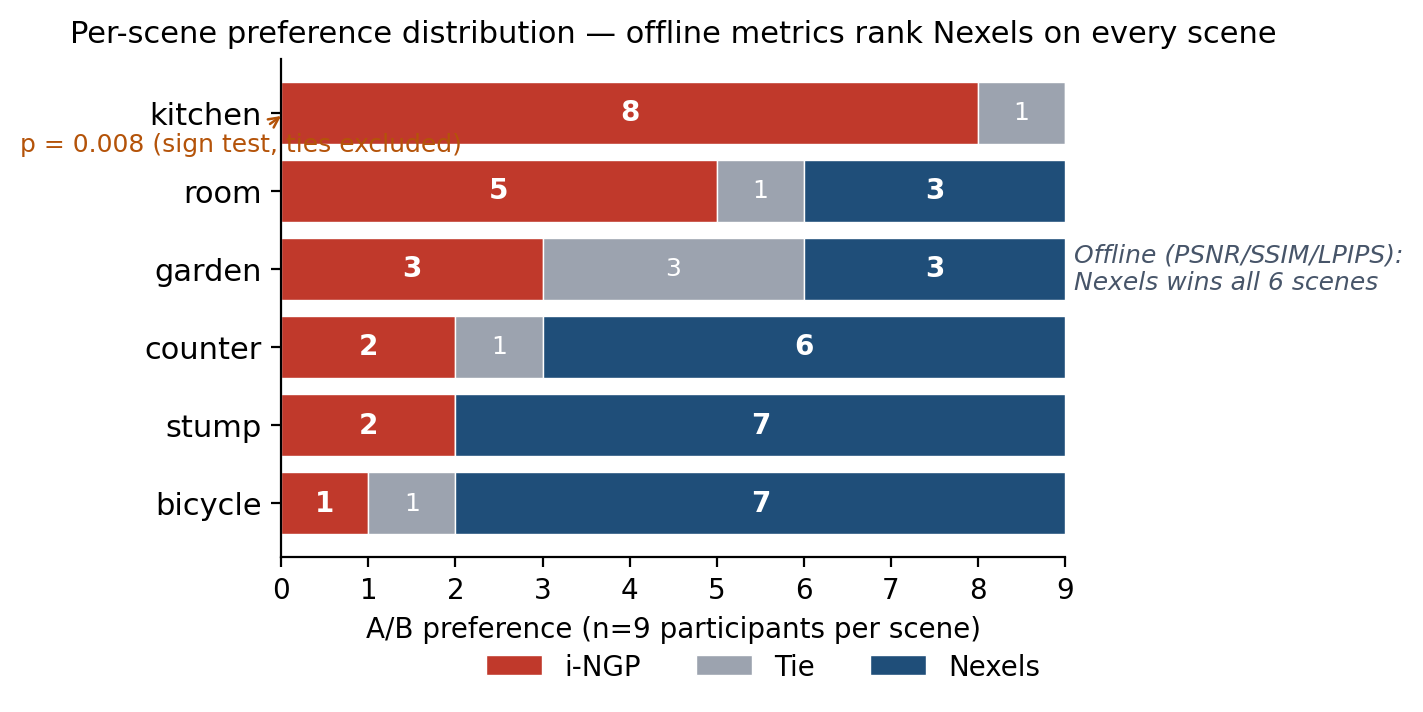
\includegraphics[width=0.85\linewidth]{fig_preference_per_scene}
  \caption{Per-scene A/B preference distribution from case study A
  ($n=18$). Each bar segments the 7-point preference scale into
  strong / moderate / slight i-NGP (red shades), tie (gray), and
  slight / moderate / strong Nexels (blue shades), so the bar's
  colour spread encodes preference \emph{strength} in addition to
  direction. Scenes ordered by net Nexels share, ascending. The
  cross-scene heterogeneity is the indication that the harness
  produces analyzable data; we do not interpret the per-scene
  rankings here.}
  \label{fig:preference_per_scene}
\end{figure}

Third, convergence-case slider trajectories across iteration counts
show non-trivial patterns (Figure~\ref{fig:convergence}). On the
smaller scene (\texttt{train}), foreground and background ratings rise
monotonically across all four checkpoints (foreground 49 $\to$ 84;
background 31 $\to$ 64), with smoothness flat after 7k. On
\texttt{truck}, the picture is more interesting: foreground saturates
between 7k and 30k (77 $\to$ 81), background flattens (72 $\to$ 72),
and \emph{smoothness drops 23 points} from 82.9 at 7k to 60.1 at 30k
--- a non-monotone trajectory that the data captures cleanly even at
$n=12$. The four checkpoint levels are clearly distinguishable, and
the data admits straightforward visual comparison against the offline
LPIPS curve overlaid on the figure.

\begin{figure}[h]
  \centering
  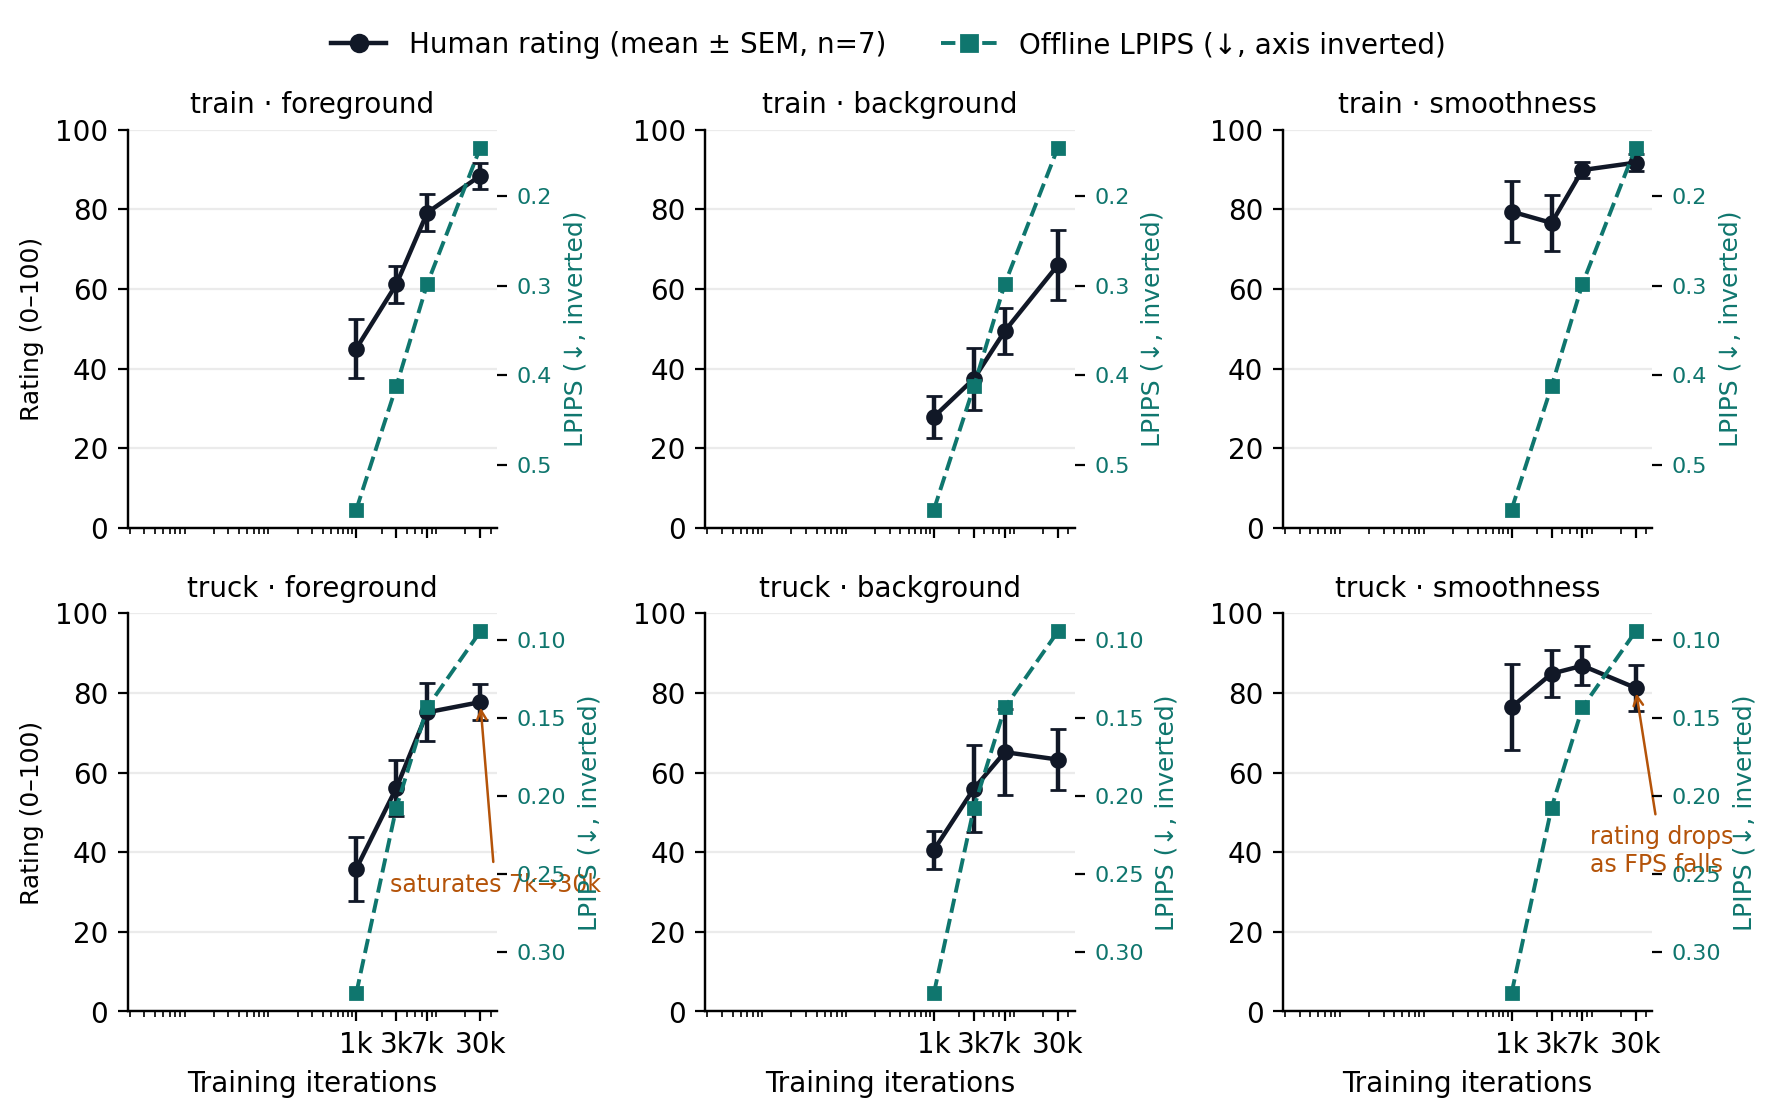
\includegraphics[width=\linewidth]{fig_convergence}
  \caption{Per-aspect mean human rating ($n=12$ participants, error
  bars are SEM) and offline LPIPS (teal dashed, axis inverted)
  across the four 3DGS checkpoints. Top row: \texttt{train}. Bottom
  row: \texttt{truck}. Columns are the three slider aspects.}
  \label{fig:convergence}
\end{figure}

These are descriptions of the data, not claims about NVS methods. A
researcher analyzing this data is the appropriate party to make
substantive claims; our role is to verify that the data has the
structure needed to support them. Appendix~\ref{app:analyses}
illustrates the kinds of analyses the data admits --- Spearman
correlations between A/B preference and offline-metric gap,
Mann--Whitney $U$ tests for aspect-citation effects, and (once
$n=18$ is large enough) Kendall's $W$ or ICC$(2,k)$ for inter-rater
agreement.

\subsection{Participant feedback}
\label{sec:participant_feedback}

This subsection addresses the participant-side success criterion via
two channels: indirect indicators from session logs, and a brief
post-session self-report survey administered to each participant.

\paragraph{Indirect indicators (from session logs).}
Every participant who loaded the viewer completed the session through
to submission: there were no mid-session abandonments in either case
study. Median session duration was approximately 9 minutes in case
study A and 5 minutes in case study B --- consistent with our piloting
estimate. No experimenter intervention was required
during any session, and no participant reported a stall, freeze, or
unresponsive UI in the post-submission notes field.

\paragraph{Post-session self-report ($n=9$).}
After each session we administer a five-question Likert survey
(1--5 scale) covering overall experience, mental fatigue, perceived
session length, instruction clarity, and ease of use of the
interactive viewer; the questionnaire itself is documented in
Appendix~\ref{app:satisfaction}. Table~\ref{tab:satisfaction} and
Figure~\ref{fig:satisfaction} summarize the $n=9$ survey responses
collected so far. The satisfaction survey was introduced partway
through recruitment so its sample lags behind the rating data;
numbers will be updated as additional survey responses come in.

\begin{table}[h]
\centering
\caption{Post-session participant survey, $n=9$ responses to date.
``Better'' indicates the direction toward positive participant
experience. Anchor conventions: overall (1 = poor, 5 = excellent);
fatigue (1 = none, 5 = a lot); length (1 = too short, 3 = just right,
5 = too long); clarity (1 = unclear, 5 = very clear); ease
(1 = hard, 5 = easy).}
\label{tab:satisfaction}
\small
\begin{tabular}{lcccl}
\toprule
Question & Better & Mean & Range & Distribution \\
\midrule
Overall experience  & $\uparrow$    & 4.44 & 4--5 & 4$\times$5, 5$\times$4 \\
Mental fatigue      & $\downarrow$  & 1.78 & 1--4 & 1$\times$4, 2$\times$4, 4$\times$1 \\
Session length feel & $\rightarrow$ & 3.11 & 3--4 & 3$\times$8, 4$\times$1 \\
Instruction clarity & $\uparrow$    & 4.44 & 4--5 & 4$\times$5, 5$\times$4 \\
Viewer ease of use  & $\uparrow$    & 3.56 & 2--5 & 2$\times$1, 3$\times$3, 4$\times$4, 5$\times$1 \\
\bottomrule
\end{tabular}
\end{table}

\begin{figure}[h]
  \centering
  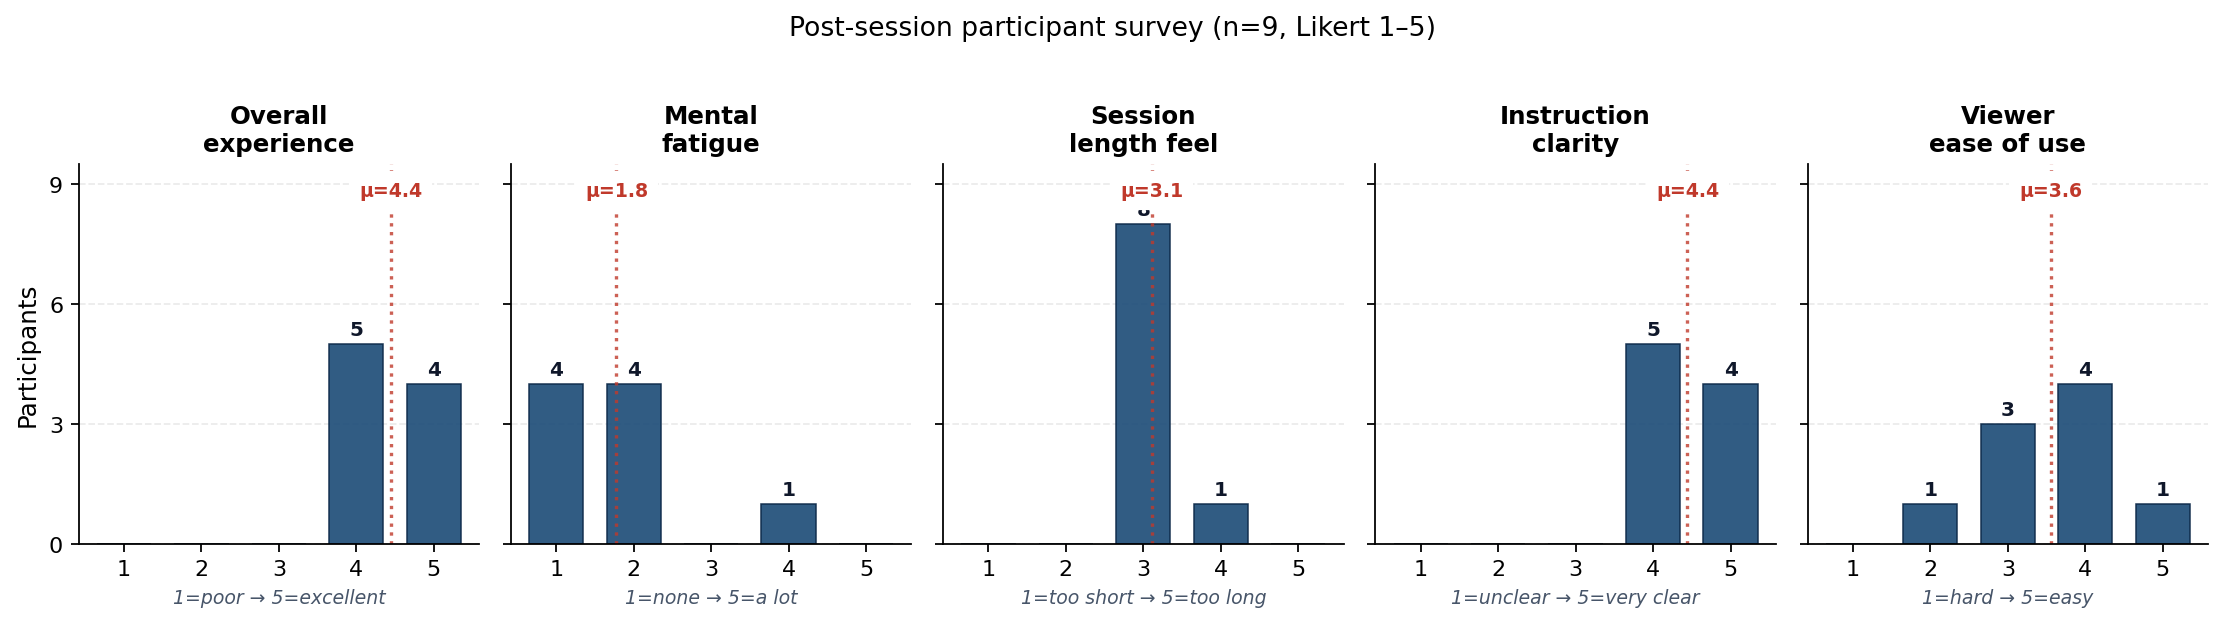
\includegraphics[width=0.95\linewidth]{fig_participant_feedback}
  \caption{Distribution of post-session participant survey responses
  ($n=9$), one histogram per question. Bar heights are participant
  counts; the dotted red line on each panel marks the mean. The
  figure will be re-rendered as the survey sample grows.}
  \label{fig:satisfaction}
\end{figure}

The signal remains positive across the board. Overall experience
sits uniformly in the 4--5 band; instruction clarity is uniformly
$\geq 4$; and 8 of 9 participants rated the session length as
``just right'' (3), with one participant rating it 4
(``a bit too long''). Mental fatigue is low (1--2) for eight of nine
respondents, with one outlier at 4. The weakest dimension is ease of
use of the interactive viewer (mean 3.56). The 2 came from the same
participant whose row also shows elevated fatigue (4), suggesting
that for at least one participant the viewer UI was itself a source
of cognitive load rather than just the rating task; a new 5 in this
column from a recent respondent pulls the mean up. With $n=9$ we
report these patterns descriptively rather than test them, and will
revisit as additional survey responses arrive.

\subsection{Limitations}
\label{sec:limitations}

The most important limitation remains sample size. At $n=18$ and
$n=12$ the statistical tests above are reasonable for the per-scene
and per-stimulus signals we surface, but underpowered for finer-grained
between-aspect comparisons; we report effect sizes alongside $p$-values
where possible. Beyond sample
size, several threats to validity warrant explicit acknowledgment.

\emph{Display variance.} Participants connected over the public
internet from uncalibrated monitors. Differences in display brightness,
gamut, and refresh rate introduce noise we cannot correct for. The
case study A design --- both methods rendered to the same participant
in the same session --- partially controls for this, but case study B
(stimuli presented sequentially) does not.

\emph{Network variance.} WebRTC adapts bitrate dynamically based on
network conditions, which means a participant on a slower network may
be evaluating a different visual stimulus than one on a faster
connection. We do not currently log per-session bitrate; for a future
version this should be instrumented and either gated or stratified.

\emph{Selection bias.} Participants were recruited from the authors'
academic environment and self-selected for interest in 3D rendering;
generalization to the broader population is not claimed.

\emph{Order and learning effects.} Case study B fixes iteration order
as ascending within scene, trading order-effect contamination for a
stable reference frame for ``better''. Case study A randomizes scene
order and A/B side assignment per pair. A first-pair learning effect
may still inflate ratings on early scenes; the \texttt{bonsai}
practice trial is intended to absorb most of this but is not a
complete control.

\emph{Method-blinding integrity.} The viewer hides method identities
behind anonymous badges. We did not collect post-hoc data on whether
participants could guess which side was which, which would be the
standard check on blinding in a perception study.

\emph{Participant-side measurement is indirect.} As described in
\S\ref{sec:participant_feedback}, our current participant-side
success indicators are entirely indirect. The planned post-session
survey is the appropriate fix, but it is not yet in the field for the
current data.

% section_4.tex — Team Responsibilities
% DRAFT for discussion — adjust attributions in concert with Ishita
% before finalizing.

\section{Team Responsibilities}
\label{sec:team}

This was a two-person project. The system, studies, and writeup were
ultimately joint products; the table below records who took primary
responsibility for each piece.

\begin{table}[h]
\centering
\small
\setlength{\tabcolsep}{6pt}
\begin{tabular}{l l}
\toprule
Responsibility & Lead \\
\midrule
\multicolumn{2}{l}{\emph{System design and implementation}} \\
\quad Overall architecture and streaming pipeline                & Connor \\
\quad Renderer wrappers (i-NGP, Nexels, 3DGS)                    & Connor \\
\quad WebSocket multiplexer and submission server                & Connor \\
\quad Viewer HTML and questionnaire UI                           & Connor \\
\quad 3DGS checkpoint training for case study B                  & Connor \\
\quad mediamtx / RTSP / WebRTC plumbing                          & Connor \\
\midrule
\multicolumn{2}{l}{\emph{Studies}} \\
\quad Questionnaire and protocol design                          & Joint \\
\quad Participant recruitment                                    & Joint \\
\quad Session administration                                     & Joint \\
\quad Post-session satisfaction survey design                    & Joint \\
\midrule
\multicolumn{2}{l}{\emph{Analysis and writing}} \\
\quad Offline-metric collection and tables                       & Connor \\
\quad Statistical analyses and figures                           & Connor \\
\quad Report drafting (\S\ref{sec:background}--\ref{sec:results}) & Joint \\
\quad Final-presentation slides                                  & Ishita \\
\quad Feedback and editorial passes on report and slides         & Joint \\
\bottomrule
\end{tabular}
\end{table}

The studies, the recruitment, the discussion of findings, and the
editorial passes on the writeup were genuinely shared, and the table's
joint rows reflect that --- we both signed off on every artifact the
project ships.

% section_appendix.tex — Systems details + example analyses
% Appended after section_3.tex; switches to appendix-style numbering.

\appendix

\section{Systems details}
\label{app:systems}

\paragraph{Per-method FPS detail.} The single-renderer FPS columns of
Tables~\ref{tab:cross_offline} and~\ref{tab:convergence} give the
per-method bench-rate ceilings at the offline benchmark resolution
(1297$\times$840). i-NGP is on average 2--3$\times$ faster than Nexels
at the \texttt{small} model size (mean 65.2 vs.\ 31.4~fps), with the
exception of \texttt{stump} where i-NGP's frame rate collapses to
27~fps for reasons related to that scene's geometry (large depth
range, many empty rays). For 3DGS, FPS scales inversely with splat
count: 434~fps at the 1k checkpoint (210k splats) drops to 77~fps at
the 30k checkpoint (1.8M splats) on \texttt{train}, and
437~$\to$~45~fps on \texttt{truck} (3.8M splats). For case study B
these numbers are all well above the 60~fps interactive target at
1920$\times$1080, so frame-rate variability inside a session was not
a confound; for case study A, both renderers cleared the 30~fps
target with substantial headroom on five of six scenes.

\paragraph{Pending telemetry.} [To be added: end-to-end input-to-photon
latency breakdown (render, encode, network, decode, display); GPU
memory residency over the course of a case-study-A session; per-renderer
frame-time distribution under cohabitation versus single-renderer
operation.]

\section{Example analyses on case-study A data}
\label{app:analyses}

The analyses below are illustrative of the kind of work a researcher
might do on data the harness collects. We present them not as
scientific claims about i-NGP or Nexels but as evidence that the data
shape supports such analyses. All numbers are computed on the $n=18$
case-study-A dataset.

\paragraph{Preference vs.\ offline-metric gaps (Spearman correlations).}
We computed Spearman correlations between A/B preference (sign
convention: $+$ Nexels preferred, $-$ i-NGP preferred) and the
per-scene gap on each offline metric (sign-aligned to ``Nexels has the
better offline number''). Table~\ref{tab:correlations} reports the
full set; Figure~\ref{fig:fps_pref_scatter} plots the scene-level
FPS--preference relationship.

\begin{table}[h]
\centering
\caption{Spearman correlation between A/B preference
($+$ Nexels / $-$ i-NGP) and per-scene offline-metric gap. Trial level
pools all (participant, scene) rows; scene-mean level averages within
scene first.}
\label{tab:correlations}
\small
\begin{tabular}{lrrrr}
\toprule
Offline-metric gap & Trial-level $\rho$ ($n=105$) & $p$ & Scene-mean $\rho$ ($n=6$) & $p$ \\
\midrule
PSNR             & $-0.06$          & $0.56$    & $-0.03$         & $0.96$    \\
SSIM             & $+0.02$          & $0.85$    & $+0.20$         & $0.70$    \\
LPIPS (AlexNet)  & $\mathbf{+0.34}$ & $\mathbf{<0.001}$ & $\mathbf{+0.83}$ & $\mathbf{0.04}$ \\
FPS              & $\mathbf{+0.35}$ & $\mathbf{<0.001}$ & $+0.77$ & $0.07$ \\
\bottomrule
\end{tabular}
\end{table}

\begin{figure}[h]
  \centering
  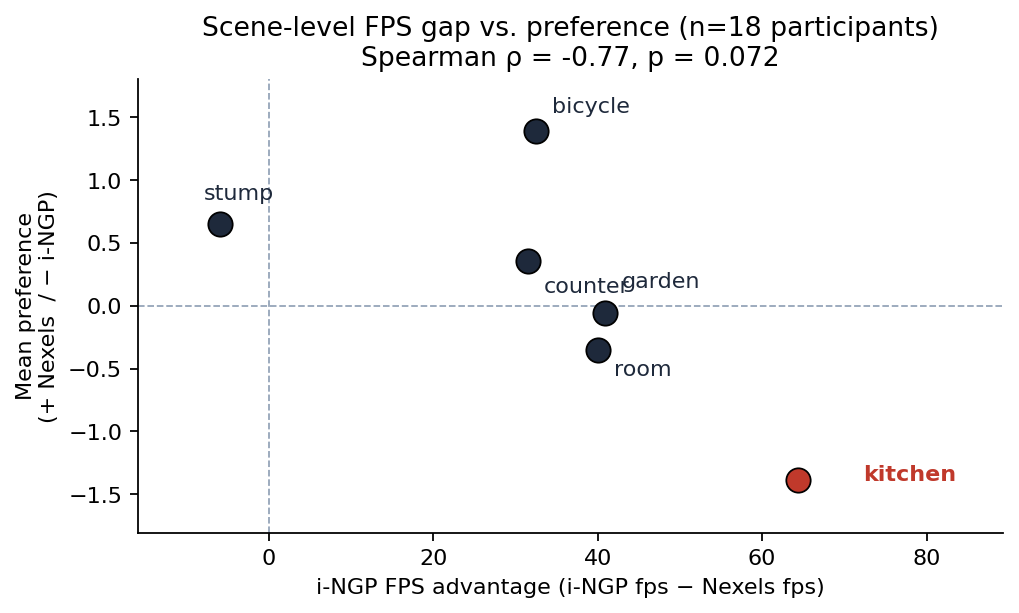
\includegraphics[width=0.85\linewidth]{fig_fps_pref_scatter}
  \caption{Per-scene mean preference ($+$ Nexels / $-$ i-NGP) plotted
  against i-NGP's FPS advantage on that scene ($n=18$ participants).
  \texttt{kitchen} is highlighted. Scene-level $\rho = -0.77$
  ($p=0.07$); trial-level $\rho = -0.35$ ($p<0.001$, $n=105$). The
  sign convention places i-NGP preference in the lower half-plane.}
  \label{fig:fps_pref_scatter}
\end{figure}

\paragraph{Aspect-citation effects (Mann--Whitney $U$).}
After each A/B choice, participants ticked which of the three aspects
(foreground, background, smoothness) influenced that choice.
Table~\ref{tab:aspect_citation} reports Mann--Whitney $U$ tests on
whether citing a given aspect changes the strength and direction of
preference. The decomposition is interpretable: background citations
correlate with stronger preferences toward Nexels; smoothness
citations with preferences toward i-NGP; foreground citations are
roughly neutral on direction. We do not over-interpret these effects;
they exemplify the within-trial decomposition the aspect multi-select
makes possible.

\begin{table}[h]
\centering
\caption{Aspect-citation effects on A/B preference. Each row tests
whether citing that aspect changes preference strength (left) or
preference direction (right). Mann--Whitney $U$ test, two-sided.}
\label{tab:aspect_citation}
\small
\begin{tabular}{lrrrrrr}
\toprule
Aspect & $|\text{pref}|$ cited ($n$) & not cited ($n$) & $p$ & signed cited & not cited & $p$ \\
\midrule
Foreground & 1.88 (57) & 1.31 (48) & $\mathbf{0.003}$ & $+0.30$ & $-0.15$ & $0.18$ \\
Background & 1.95 (59) & 1.20 (46) & $\mathbf{<0.001}$ & $\mathbf{+0.63}$ & $\mathbf{-0.59}$ & $\mathbf{<0.001}$ \\
Smoothness & 2.09 (34) & 1.39 (71) & $\mathbf{<0.001}$ & $\mathbf{-0.62}$ & $\mathbf{+0.44}$ & $\mathbf{0.009}$ \\
\bottomrule
\end{tabular}
\end{table}

\begin{figure}[h]
  \centering
  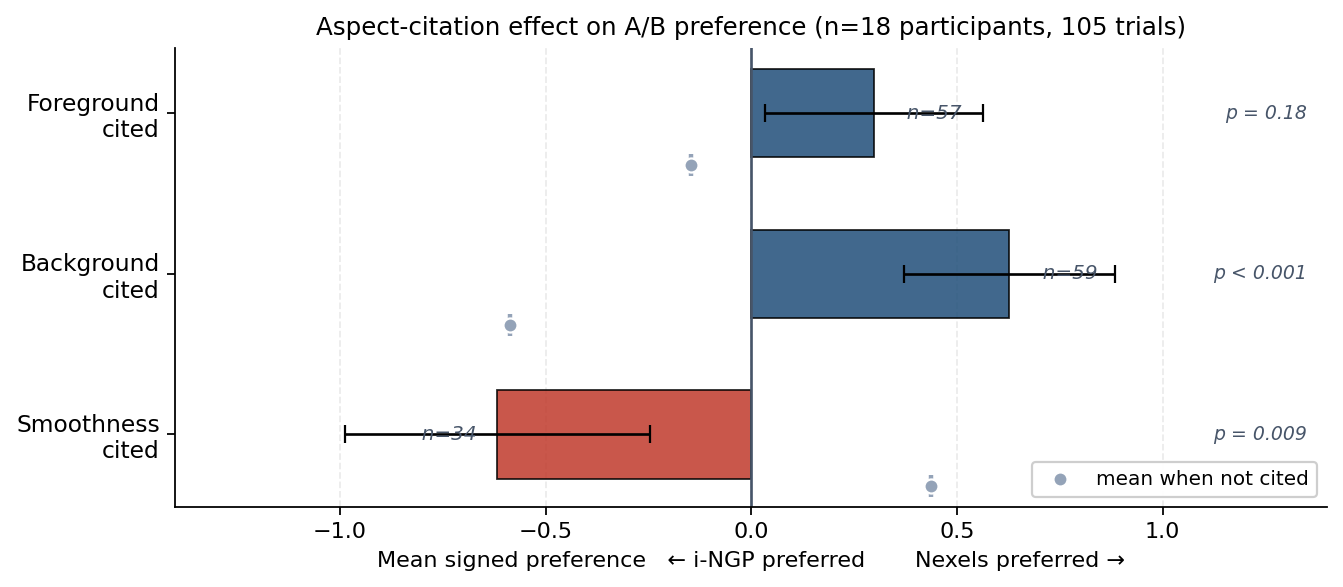
\includegraphics[width=0.85\linewidth]{fig_aspect_citation}
  \caption{Visualization of the direction column of
  Table~\ref{tab:aspect_citation}: mean signed A/B preference on
  trials where each aspect was cited (bars; red = pulls toward
  i-NGP, blue = pulls toward Nexels), with the corresponding
  not-cited mean shown as a gray marker for contrast. Citing
  background pulls preference toward Nexels; citing smoothness pulls
  it toward i-NGP; foreground citations are roughly neutral on
  direction. Error bars are SEM.}
  \label{fig:aspect_citation}
\end{figure}

\paragraph{Per-scene breakdown.}
Table~\ref{tab:aspect_per_scene} resolves
Table~\ref{tab:aspect_citation} one level further by splitting each
aspect's citation count by both scene and the direction the citer
chose. The column-total row exposes an asymmetry that the aggregate
table cannot: Nexels-choosing citers invoke smoothness only 12 times
across all six scenes, against 33--38 for foreground and background;
i-NGP-choosing citers invoke all three aspects nearly equally
(24/21/22). Participants who chose Nexels were almost always doing
so on the strength of \emph{what they saw}; participants who chose
i-NGP did so on the strength of what they saw \emph{and} how it
moved.

\begin{table}[h]
\centering
\caption{Per-scene aspect citations split by A/B preference direction.
Each cell counts trials where the row's aspect was cited \emph{and}
the participant chose the column's method. No tied participant cited
any aspect, so a third column group is unnecessary. Bold marks the
largest cell per scene within the winning column group.}
\label{tab:aspect_per_scene}
\small
\begin{tabular}{l@{\quad}rrr@{\quad}rrr}
\toprule
       & \multicolumn{3}{c}{i-NGP citers} & \multicolumn{3}{c}{Nexels citers} \\
\cmidrule(lr){2-4} \cmidrule(lr){5-7}
Scene  & fg & bg & sm & fg & bg & sm \\
\midrule
bicycle & 1 & 0 & 2 & 8 & \textbf{11} & 3 \\
counter & 3 & 4 & 3 & \textbf{7} & 6 & 1 \\
garden  & 3 & 2 & 4 & 2 & \textbf{7} & 3 \\
kitchen & \textbf{8} & 5 & 7 & 2 & 1 & 0 \\
room    & \textbf{8} & 5 & 5 & 4 & 5 & 2 \\
stump   & 1 & 5 & 1 & \textbf{10} & 8 & 3 \\
\midrule
\textbf{total} & 24 & 21 & 22 & 33 & \textbf{38} & 12 \\
\bottomrule
\end{tabular}
\end{table}

\paragraph{Instrument internal consistency.}
Per-row slider gaps (Nexels rating minus i-NGP rating on each aspect)
correlate with the same row's A/B preference at $\rho = 0.65$
(foreground), $0.71$ (background), and $0.60$ (smoothness), all
$p < 10^{-10}$ at $n=105$. When participants rate the methods
differently on a continuous slider, that flows through cleanly to
their forced choice on the same trial --- the two instruments measure
compatible things.

\paragraph{Inter-rater agreement.}
At $n=18$ standard inter-rater agreement metrics (Kendall's $W$ on
A/B preference per scene; ICC$(2,k)$ on per-aspect slider scores)
become computable with usefully narrow confidence intervals. We
defer the specific numbers to a follow-up pass.

\section{Post-session participant satisfaction questionnaire}
\label{app:satisfaction}

We administer the following five-question Likert survey (Google Forms,
1--5 scale) after each rating session. The survey is intentionally
short --- five multiple-choice items --- to keep response rate high;
qualitative comments are already captured by the rating viewer's
notes field, so this post-session instrument is purely quantitative.

\begin{enumerate}
    \item \textit{Overall, how was your participant experience?}
    \quad(1 = poor $\rightarrow$ 5 = excellent)
    \item \textit{By the end of the session, how mentally fatigued
    did you feel?} \quad(1 = not at all $\rightarrow$ 5 = a lot)
    \item \textit{How long did the length of the session feel?}
    \quad(1 = too short, 3 = just right, 5 = too long)
    \item \textit{How clear were the instructions and questions for
    the tasks?} \quad(1 = unclear $\rightarrow$ 5 = very clear)
    \item \textit{How easy was it to use the interactive viewer?}
    \quad(1 = hard $\rightarrow$ 5 = easy)
\end{enumerate}

The five items together cover the four facets of participant-side
success defined in \S\ref{sec:success}: overall experience (Q1);
cognitive load and pacing (Q2, Q3); task interpretability (Q4); and
UI quality (Q5). Aggregated results to date appear in
\S\ref{sec:participant_feedback}.

% \input{section_5}  % References — emit via \bibliography below

\bibliographystyle{plainnat}
\bibliography{refs}

\end{document}
